\chapter{Aerosol Physics}
\labelchapter{physics}

In this chapter we describe the physics of aerosols as represented by Haero's
modal aerosol model. First, we review the modal aerosol approximation, which
defines the equations and quantites of interest and describes how various
aerosol processes are parameterized. Then we describe in detail these various
parameterized aerosol processes, their physical significance, and their
mathematical represention. Along the way, we take care to highlight any
physical, statistical, and mathematical assumptions, to make clear the
circumstances under which Haero's aerosol model is valid.

\section{The Modal Aerosol Approximation}

Here we offer an extremely abbreviated ``fly-over'' of the evolution equations
that quantify the dynamics of aerosols. Here, we emphasize the mathematical
representation of aerosols. For a more detailed explanation of the underlying
ideas, we refer the reader to~\cite{Whitby1991} and~\cite{Friedlander1977}.

All quantities are in SI units unless specifically mentioned. To keep the
discussion simple and focused, we avoid referencing specific coordinates.

Many of the assumptions here are inherited from Dick Easter's Modal Aerosol
Model 4-mode (MAM4) model.

\subsection*{Size Matters}

The modal approach to modeling aerosols is based on the observations that

\begin{itemize}
  \item the sizes of aerosol particles greatly influence their dynamical
        behavior
  \item these sizes span several orders of magnitude (from 0.001 to 100 microns)
\end{itemize}

Here, a ``particle'' is an individual aerosol molecule with some volume $V_p$.
Aerosol particles consist of polymers, and a particle consisting of a chain of
$i$ monomers is an $i$-mer.

How do we represent a set of aerosol particles in space, given the importance
of their size? In the simplest case (for small $i$-mers), we can denote
$N_i(\vec{x}, t)$ as the number of $i$-mers per cubic meter in the vicinity of
the point $\vec{x}$ at time $t$. In this language, the evolution equation is a
set of coupled advection-diffusion-reaction (ADR) equations acting under the
influence of a bulk velocity $\vec{v}$:

\begin{equation}\labeleq{small_imer_dNdt}
  \ddt{N_i} + \div{(N_i\vec{v})} = \mathcal{D}(\nabla N_i) +
                                   \mathcal{R}(\{N_j\}) +
                                   \mathcal{S}(N_i, t)
\end{equation}

Here we represent terms on the right hand side by

\begin{itemize}
  \item $\mathcal{D}$: terms related to {\it diffusion processes} for $N_i$
  \item $\mathcal{R}$: terms related to {\it reaction processes}, in which
        various $j$-mers combine, react, and dissociate to form particles of
        other types
  \item $\mathcal{S}$: terms related to {\it source and sink processes},
        including external and prescribed sources of $N_i$.
\end{itemize}

We describe the forms of these terms in \refsection{processes}. The bulk
velocity $\vec{v}$ is supplied by some dynamical atmospheric model.

For larger $i$-mers ($i > 100$), the above description becomes inadequate, and
we must adopt a description for particle numbers that admits a continuous
number distribution in particle size space.

Let $n(V_p, \vec{x}, t)$ be the number of particles of volume $V_p$ occupying
the point $\vec{x}$ at time $t$. Then the evolution of all $i$-mers is described
by a single ADR equation:

\begin{equation}\labeleq{continuous_dndt}
  \ddt{n} + \div{(n\vec{v})} = \mathcal{D}(\nabla n) +
                               \mathcal{R}(n) +
                               \mathcal{S}(n, t)
\end{equation}

where $\mathcal{D}$, $\mathcal{R}$, and $\mathcal{S}$ have been expressed
in terms of $n$ instead of $N_i$. This is a tidy equation, but $n$ is a
number distribution function that introduces a new dimension---the particle volume
$V_p$---to the solution space. This makes it inconvenient for doing numerical
calculations. In this description, $n$ can assume any shape in particle volume
space, which raises the question of how to constrain the solution in $V_p$.

\subsection*{Moment Equations and the Closure Problem}
We can reduce the size of our solution space by making a few assumptions:

\begin{assume}
  The detailed structure of the number distribution function
        $n(V_p, \vec{x}, t)$ is unimportant to aerosol dynamics.
\end{assume}

If we don't need to obtain the full solution for $n$, we can select a specific
functional form $n(D_p, \vec{x}, t) = n(\vec{x}, t; D_p)$ for it. Then, taking cues from
methods in particle kinetics and turbulence theory, we can integrate the product
of \refeq{continuous_dndt} with powers of $D_p$ to obtain the {\bf moment
equations}

\begin{equation}\labeleq{moments}
  \ddt{\mathcal{M}_k} + \div{(\mathcal{M}_k\vec{v})} = \int_0^{\infty} D_p^k (\mathcal{D} + \mathcal{R} + \mathcal{S}) \d{D_p}
\end{equation}

where $\mathcal{M}_k(\vec{x}, t) = \int_0^{\infty} D_p^k n(\vec{x}, t; D_p) \d{D_p}$
is the ``$k$th moment'' of $n$.

The moment equations are solved by picking a specific form of $n$'s functional
dependence on $D_p$ and playing tricks to avoid actually evaluating the
above integrals. However, the moment equations aren't closed---the advection,
diffusion, reaction, and source terms can all involve $n$ and its spatial
derivatives, and in general, the evolution of $\mathcal{M}_k$ is coupled to higher
moments. To make further progress, we must solve this {\bf closure problem}.

\subsection*{Modal Equations}

Having already given up on obtaining a general solution for $n(\vec{x}, t)$,
we allow ourselves to make another assumption:

\begin{assume}[Modal assumption]
  The number distribution function $n$ is the sum of a set of
        specific number distribution functions $n_i$, each representing a
        {\bf mode} with a specific functional form for a sub-population of
        aerosol particles occupying a certain range in particle size space.
\end{assume}
In other words,

\begin{equation}\labeleq{modal_n}
  n(\vec{x}, t; D_p) = \sum_{i=1}^M n_i(\vec{x}, t; D_p)
\end{equation}

where $n_i$ represents aerosol particles with sizes falling within the range
of mode $i$ and $M$ is the number of modes. Each mode assumes a specific
functional form for $n_i$ in terms of its relevant size as given by $D_p$.
We include the arguments $\vec{x}$ and $t$ to emphasize that this equation holds
at each point in space and at each instant in time for an aerosol system.

\subsubsection*{Log-Normal Distribution Functions}

Haero constructs its multi-modal distribution functions from log-normal
probability distribution functions (PDFs) for each mode $i$. The PDF for mode
$i$ expresses the fraction of aerosol particles present per unit size interval,
in terms of a continuous particle diameter $D_p$ within that mode. Such PDFs
have been found to represent measured aerosol size distributions with a level of
accuracy comparable to that of the relevant measurement
techniques~\cite{Whitby1991}.

\begin{assume}[Log-normal PDF]
The probability distribution function $f_i$ used to construct
        the number distribution function $n_i$ for mode $i$ is a continuous
        function of the particle diameter $D_p$, given as a log-normal distribution,
        \begin{equation}\labeleq{log_normal_pdf}
  f_i(D_p) = \frac{1}{\sqrt{2\pi} D_p \ln \sigma_{g,i}} \ 
      \exp \left [-\frac{(\ln D_p - \ln D_{g,i})^2}{2\ln^2 \sigma_{g,i}} \right]
\end{equation}
where we have introduced the geometric mean $D_{g,i}$ and the geometric standard
deviation $\sigma_{g,i}$ of $D_p$ within mode $i$. 

\end{assume}

In general, these two parameters are determined for each mode via moment equations and corresponding time-evolution equations.
Haero makes an additional simplifying assumption:

\begin{assume}[Constant standard deviation]
  The geometric standard deviation $\sigma_{g,i}>1$ for each mode $i$ is constant in time.  
  The justification for this assumption in \cite{Easter2004,Wilson2001,Whitby1991} is given in \cite{Whitby1981}.
\end{assume}


This PDF can also be expressed in ``logarithmic form'' in terms of $\ln D_p$
of $D_p$:
\begin{equation}\label{eq:log_normal_pdf_log}
  g_i(\ln D_p) = \frac{1}{\sqrt{2\pi} \ln\sigma_{g,i}} \
      \exp \left [ -\frac{(\ln D_p - \ln D_{g,i})^2}{2\ln^2 \sigma_{g,i}} \right]
\end{equation}

Here, $g_i$ is a normal distribution of $\ln D_p$ with a mean of $\ln D_{g,i}$
and standard deviation of $\ln\sigma_{g,i}$.

These PDFs are referred to as {\bf normalized size distribution functions} in
Haero. We can justify this name by multiplying each PDF by the total particle
number density $N_i$ for mode $i$ to obtain the equivalent number distribution
functions:

\begin{align}\label{eq:log_normal_n}
  n_i(D_p) = N_i f_i(D_p) &= \frac{N_i}{\sqrt{2\pi} D_p \ln \sigma_{g,i}} \ 
  \exp \left [ - \frac{(\ln D_p - \ln D_{g,i})^2}{2\ln^2\sigma_{g,i}} \right ] \\
  \hat{n}_{i}(\ln D_p) = N_i g_i(\ln D_p) &= \frac{N_i}{\sqrt{2\pi}\ln \sigma_{g,i}} \ 
	\exp \left [ - \frac{(\ln D_p - \ln D_{g,i})^2}{2\ln^2\sigma_{g,i}} \right ]
\end{align}

\begin{figure}
\centering
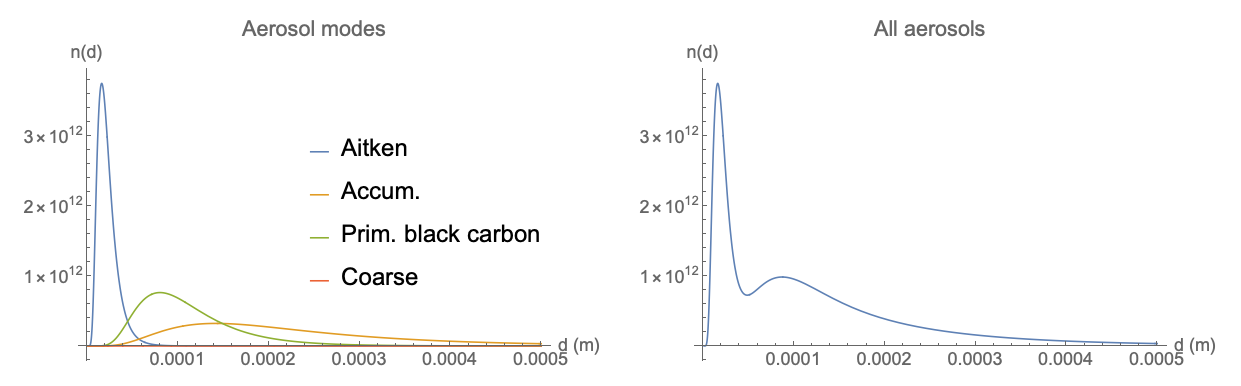
\includegraphics[width=\textwidth]{figures/pdf_examples}
\caption{Normalized size distributions $n_i$ for each mode in the Haero model
with $N_i$ set by the \texttt{num\_aer} variable.}\label{fig:mode_dists}
\end{figure}

The logarithmic form $\hat{n}_i$ is useful because of the relationship
$ n_i(D_p) = \hat{n}_i(\ln D_p)/D_p$, which allows us to write
\begin{equation} \labeleq{equ_norm_lognorm}
  n_i(D_p) \d{D_p} = \hat{n}_i(\ln D_p) \d{\ln D_p}
\end{equation}
to simplify integrands involving number distribution functions.
The benefit of this log-normal functional form choice is that the moment integrals can be defined analytically, obviating the need for potentially costly numerical quadrature \cite[eqns.~(3.7)]{Whitby1991}.
The $k$th moment is given in this case by,
\begin{equation}
  M_k^{(i)} = N_i D_{g,i}^k \exp\left(\frac{k^2}{2}\log^2\sigma_{g,i}\right).
\end{equation}

In particular,
\begin{subequations}
  \begin{align}
    M_0^{(i)} &= \int_0^\infty n_i(D_p)\,d D_p = N_i,\\
    M_1^{(i)} &= \int_0^\infty D_p n_i(D_p)\,d D_p = N_iD_{g,i}\exp({\frac{1}{2}\log^2\sigma_{g,i}}),\\
    M_2^{(i)} &= \int_0^\infty D_p^2n_i(D_p)\,d D_p = N_iD_{g,i}^2\exp(2\log^2\sigma_{g,i}),\\
    M_3^{(i)} &= \int_0^\infty D_p^3n_i(D_p)\,d D_p = N_iD_{g,i}^3\exp(\frac{9}{2}\log^2\sigma_{g,i})
  \end{align}
\end{subequations}


\begin{defn}[Particle size]
  Particle size $\overline{D_i}$ for the $i$th mode is defined by the arithmetic mean diameter associated with the 3rd moment \cite[eqn.~(1)]{Whitby1981}, 
  \begin{equation}
    \overline{D_i} = \left(M_3^{(i)}/N_i)\right)^{1/3} = D_{g,i}\exp\left(\frac{3}{2}\log^2\sigma_{g,i}\right)
  \end{equation}
\end{defn}

\begin{assume}[Particles have spherical shapes] Aerosol particles are spherical, and their size can be parameterized by their diameter $\overline{D_i}$.
The corollaries for area and volume follow, $\overline{A_i} = \pi\overline{D_i}^2$, $\overline{V_i} = \frac{\pi}{6}\overline{D_i}^3$.
\end{assume}
\pbc{I can't make a consistent $\overline{D_i}$ work with more than one $k>0$ moment. Indeed, even \cite[eqn.~(1)]{Whitby1981} notes that this choice must be associated with a specific moment. 
To see this, check: 
$$\overline{D_i}^3 \ne M_3^{(i)}/N_i. $$
The factors multiplying $\log^2\sigma_{g,i}$ do not match.
\\
Perhaps we get away with this incongruity because MAM really only used $M_{0,3}^{(i)}$ and ignores the first and second moments?
}


%\pbc{I've verified the above equations (11), which correspond to \cite[eqns.~(3.7)]{Whitby1991}, but I haven't yet figured out how they relate to $\bar A_i$, $\bar D_i$, and $\bar V_i$, unless: 
%  $$\overline{D_i} = D_{g,i}\exp(\frac{1}{2}\log^2\sigma_{g,i}),~~\overline{A}_i = \pi D_{g,i}^2\exp(2\log^2\sigma_{g,i}),~~ \overline{V_i} = \frac{\pi}{6}D_{g,i}^3\exp(\frac{9}{2}\log^2\sigma_{g,i}).$$
%  In any case, I don't know where the constant exponential factors go.
%  They remain, for example, in \cite[eqn.~(1)]{Whitby1981}.
%}

When we adopt the log-normal assumption, we express our solution for particles in
mode $i$ in terms of its zeroth, first, second, and third moments
$\mathcal{M}_k^{(i)}(\vec{x}, t)$. These are, respectively:
\begin{itemize}
  \item $\mathcal{M}_0^{(i)} = N_i$, the total number of concentration for particles
        in mode $i$
  \item $\mathcal{M}_1^{(i)} = N_i\overline{D}_i$, the number-weighted mean diameter of
        particles in mode $i$
  \item $\mathcal{M}_2^{(i)} = \frac{1}{\pi}N_i\overline{A}_i$, a number-weighted
        surface area of particles in mode $i$
  \item $\mathcal{M}_3^{(i)} = \frac{6}{\pi}N_i\overline{V}_i$, a number-weighted
        volume of particles in mode $i$
\end{itemize}

In this language, the aerosol evolution equation for the $k$th moment of the
$i$th mode is

\begin{equation}\labeleq{modal_evolution}
  \ddt\mathcal{M}_k^{(i)} = F_k^{(i)}(N_i, \overline{D}_i, \overline{A}_i, \overline{V}_i, T, p, \mathsf{...})
\end{equation}

where the air temperature $T$ and the air pressure $p$ enter the moment
equations, via right hand side terms in \refeq{moments}. These are the
{\bf modal equations}.

\begin{assume}[Parmeterization assumption]
   The time evolution of a moment $\mathcal{M}_k^{(i)}$ can be
    expressed in terms of the quantities $N_i$, $\overline{D}_i$,
    $\overline{A}_i$, $\overline{V}_i$, the air temperature $T$, the pressure $p$, and a few
    selected additional quantities.
\end{assume}

\begin{assume}[2-moment scheme]
  Aerosol dynamics can be represented well by two moments, $M_0^{(i)}$ and $M_3^{(i)}$.
  We therefore need to find equations that describe the time evolution of $M_0^{(i)}$ and $M_3^{(i)}$ in terms of known E3SM variables.
  \begin{itemize}
    \item The number of moles of aerosol per kg of air is $N_i/N_A$, where $N_A$ is the Avogadro Constant.
    \item The mass mixing ratio of aerosol (kg aer.\,/ kg air) is therefore $\displaystyle q^{(i)} = \frac{N_i M_w}{N_A} = \frac{\mathcal{M}_0^{(i)}M_w}{N_A}$, where $M_w$ is the molecular weight (kg/mol) of the aerosol particles in mode $i$.
    \item The mass density of aerosol particles in mode $i$ is therefore, $\rho_{aer}^{(i)} =\rho_{air} \;q^{(i)}$.
    \item The total mass of aerosol particles is then $\displaystyle M_{aer}^{(i)}=\rho_{aer}^{(i)} \overline{V_i} = \frac{\pi}{6}\frac{\rho_{aer}^{(i)}\mathcal{M}_3^{(i)}}{\mathcal{M}_0^{(i)}}$.
  \end{itemize}
\end{assume}

%Solving the closure problem is then reduced to finding expressions for
%$\overline{D}_i$, $\overline{A}_i$, and $\overline{V}_i$ that relate the
%different moments of $n_i$:
%
%\begin{align}
%  \overline{D}_i &= \overline{D}_i(\mathcal{M}_{k_1}^{(i)}/N_i, \mathcal{M}_{k_2}^{(i)}/N_i) \labeleq{D_i}\\
%  \overline{A}_i &= \overline{A}_i(\mathcal{M}_{k_1}^{(i)}/N_i, \mathcal{M}_{k_2}^{(i)}/N_i) \labeleq{A_i}\\
%  \overline{V}_i &= \overline{V}_i(\mathcal{M}_{k_1}^{(i)}/N_i, \mathcal{M}_{k_2}^{(i)}/N_i) \labeleq{V_i}
%\end{align}
%
%Here, we formulate the above expressions by the selecting pairs of moments that
%contribute to the evolution of each quantity for mode $i$.
%
%\begin{assume}[Moment pairs]
% The averaged quantities $\overline{D}_i$, $\overline{A}_i$,
%    and $\overline{V}_i$ can each be expressed as a function of a pair of
%    specific number-normalized moments for the $i$th mode.
%\end{assume}

\subsubsection*{Mode definitions in MAM4}

The choices of size range and width for the modes in MAM are based on
measurements of tropospheric aerosols (see~\cite{Easter2004} and references therein).
Table~\ref{tab:mode_size_parameters} shows the relevant parameters for MAM4,
the 4-mode legacy MAM model.

%------------------- table: mode parameters ---------------
\begin{table}[htbp]
\centering
%\caption{
%Geometric mean dry diameter ($D\dsub{gn,d,i}$, unit:
%$\rm \mu m$) and geometric standard deviation ($\sigma\dsub{g,i}$)
%of the number size distribution of each log-normal mode.
%}
%\begin{tabular}{ccccc}
%  \toprule
%  Mode        &  Lower bound of $D\dsub{gn,d,i}$  &  $D\dsub{gn,d,i}$   &
%  Upper bound of $D\dsub{gn,d,i}$  &  $\sigma\dsub{g,i}$ \\
%  \midrule
%  Aitken 	            &  0.0087  &   0.026   &   0.052  &  1.6 \\
%  Accumulation     &  0.0535  &   0.11      &   0.44    &  1.8 \\
%  Coarse               &  1.0        &   2.0       &   4.0      &  1.8 \\
%  Primary carbon  &  0.01      &   0.05      &   0.1      &  1.6 \\
%  \bottomrule
%\end{tabular}
\caption{Parameters of log-normal modes in MAM4.}
\label{tab:mode_size_parameters}
\begin{tabular}{cccccc}
  \toprule
  Mode           &  Lower bound of $D\dsub{gn,d,i}$
                 &  Upper bound of $D\dsub{gn,d,i}$  &  $\sigma\dsub{g,i}$ 
                 & $N_i(0)$\\
  \midrule
  Aitken 	 &  0.0087  &   0.052  &  1.6     & 7.9031E7\\
  Accumulation   &  0.0535  &   0.44   &  1.8 & 7.9697E7\\
  Coarse         &  1.0     &   4.0    &  1.8 & 8.0361E7\\
  Primary carbon &  0.01    &   0.1    &  1.6 & 8.1022E7\\
  \bottomrule
\end{tabular}
\end{table}
%-------------

Thus, in MAM, all modes have the same mathematical form, but the parameters
are different for each mode.

\subsection*{Multi-Species Modes}

We have derived the modal equations assuming that each mode contains a
population of undifferentiated aerosol particles. 
We assume that each particle is composed of several, potentially different, chemical species, which corresponds to the following assumption.
%If we wish to track individual
%particle species within a mode, we may do so by expressing the population of a
%mode as the sum of its constituent species in the modal assumption, adding
%a species index $s$ to the number distribution function $n$:
%
%\begin{equation}\labeleq{modal_multi_species}
%  n(\vec{x}, t; D_p) = \sum_{i=1}^M \sum_{s=1}^S n_{i,s}(\vec{x}, t; D_p)
%\end{equation}
%
%with $S$ as the number of species. Then we can carry out the subsequent analysis
%as before, breaking up the moments into species-specific parts
%$\mathcal{M}_k^{(i,s)}$ and expressing the total $k$th moment as the sum of these
%parts:
%
%\begin{equation}
%  \mathcal{M}_k^{(i)} = \sum_{s=1}^S \mathcal{M}_k^{(i,s)}
%\end{equation}
%
%Then the multi-species modal evolution equations are
%
%\begin{equation}\labeleq{modal_multi_species_evolution}
%  \ddt\mathcal{M}_k^{(i,s)} = F_k^{(i,s)}(N_{i,s}, \overline{D}_{i,s}, \overline{A}_{i,s}, \overline{V}_{i,s}, T, p, \mathsf{...})
%\end{equation}
%
%with species-specific equivalents of the quantities in \refeq{modal_evolution}.

\begin{assume}[Internally mixed]
  All aerosol species within a mode are assumed to be carried uniformly by all particles represented by the mode's log-normal distribution function, i.e., within each mode, particles are internally mixed.
\end{assume}

\begin{assume}[Additive particle volume]
  Quantitatively, the internal mixing assumption implies that the volume of each individual particle is the sum of the volumes of its various constituents; in this case, the species within the mode.  
\end{assume}

These assumption has several implications:
\begin{enumerate}
  \item All species within mode $i$ share the same particle size distribution; as a corollary, they also share the same number concentration,
  \begin{equation}
    N_{i,q} = M_0^{(i)} = N_i,
  \end{equation}
  for all species $q$ in mode $i$.
\end{enumerate}

